\documentclass[letterpaper,10pt]{article}
\usepackage[pdftex]{graphicx}
\usepackage{listings}
\usepackage{alltt}
\usepackage{color}
\usepackage{amsmath}
\usepackage{hyperref}
\usepackage{pgfplotstable}
\usepackage{float}

\definecolor{dkgreen}{rgb}{0,0.6,0}
\definecolor{gray}{rgb}{0.5,0.5,0.5}
\definecolor{mauve}{rgb}{0.58,0,0.82}

\hypersetup{
    colorlinks,
    citecolor=black,
    filecolor=black,
    linkcolor=black,
    urlcolor=black
}

\lstset{
	basicstyle=\footnotesize,
	breaklines=true,
	 backgroundcolor=\color{white},   % choose the background color; you must add \usepackage{color} or \usepackage{xcolor}
  basicstyle=\footnotesize,        % the size of the fonts that are used for the code
  breakatwhitespace=false,         % sets if automatic breaks should only happen at whitespace
  breaklines=true,                 % sets automatic line breaking
  captionpos=b,                    % sets the caption-position to bottom
  commentstyle=\color{dkgreen},    % comment style
  deletekeywords={...},            % if you want to delete keywords from the given language
  escapeinside={\%*}{*)},          % if you want to add LaTeX within your code
  extendedchars=true,              % lets you use non-ASCII characters; for 8-bits encodings only, does not work with UTF-8
  frame=single,	                   % adds a frame around the code
  keepspaces=true,                 % keeps spaces in text, useful for keeping indentation of code (possibly needs columns=flexible)
  keywordstyle=\color{blue},       % keyword style
  otherkeywords={*,grep,sort,head,mv,perl,chmod,...},           % if you want to add more keywords to the set
  numbers=left,                    % where to put the line-numbers; possible values are (none, left, right)
  numbersep=5pt,                   % how far the line-numbers are from the code
  numberstyle=\tiny\color{gray}, % the style that is used for the line-numbers
  rulecolor=\color{black},         % if not set, the frame-color may be changed on line-breaks within not-black text (e.g. comments (green here))
  showspaces=false,                % show spaces everywhere adding particular underscores; it overrides 'showstringspaces'
  showstringspaces=false,          % underline spaces within strings only
  showtabs=false,                  % show tabs within strings adding particular underscores
  stepnumber=1,                    % the step between two line-numbers. If it's 1, each line will be numbered
  stringstyle=\color{mauve},     % string literal style
  tabsize=2,	                   % sets default tabsize to 2 spaces
  title=\lstname                   % show the filename of files included with \lstinputlisting; also try caption instead of title
}


\begin{document} 

\begin{titlepage}

\begin{center}

\Huge{Assignment 5}

\Large{CS532-s16:  Web Sciences}

\Large{Spring 2016}

\Large{John Berlin}

\Large Generated on \today

\end{center}

\end{titlepage}
\newpage
\section*{1}
\subsection*{Question}
\begin{verbatim}
We know the result of the Karate Club (Zachary, 1977) split.
Prove or disprove that the result of split could have been predicted
by the weighted graph of social interactions.  How well does the
mathematical model represent reality?

Generously document your answer with all supporting equations, code,
graphs, arguments, etc.

Useful sources include:

* Original paper

http://aris.ss.uci.edu/~lin/76.pdf

* Slides

http://www-personal.umich.edu/~ladamic/courses/networks/si614w06/ppt/lecture18.ppt

http://clair.si.umich.edu/si767/papers/Week03/Community/CommunityDetection.pptx

* Code and data

http://networkx.github.io/documentation/latest/examples/graph/karate_club.html

http://nbviewer.ipython.org/url/courses.cit.cornell.edu/info6010/resources/11notes.ipynb

http://stackoverflow.com/questions/9471906/what-are-the-differences-between-community-detection-algorithms-in-igraph/9478989#9478989

http://stackoverflow.com/questions/5822265/are-there-implementations-of-algorithms-for-community-detection-in-graphs

http://konect.uni-koblenz.de/networks/ucidata-zachary

http://vlado.fmf.uni-lj.si/pub/networks/data/ucinet/ucidata.htm#zachary

https://snap.stanford.edu/snappy/doc/reference/CommunityGirvanNewman.html

http://igraph.org/python/doc/igraph-pysrc.html#Graph.community_edge_betweenness
\end{verbatim}
\newpage
\subsection*{Answer}
Before proving whether or not the result of split could have been predicted, let us first understand the problem. Zachary's Karate Club \cite{zacharykclub} is a very well known graph problem, where the social interactions between two groups ``\emph{Mr. Hi} and \emph{John A}", caused a split in that social community. The club as seen in figure \ref{fig:zkc} is the original club with the results of the split shaded according to which faction each member went too. As seen in figure \ref{fig:zkc}, the graph(club) is highly connected, which leaves us to wonder how would we figure out how to predict the division solely using the graph itself.

\begin{figure}[htbp]%https://en.wikibooks.org/wiki/LaTeX/Floats,_Figures_and_Captions#Figures
\begin{center}
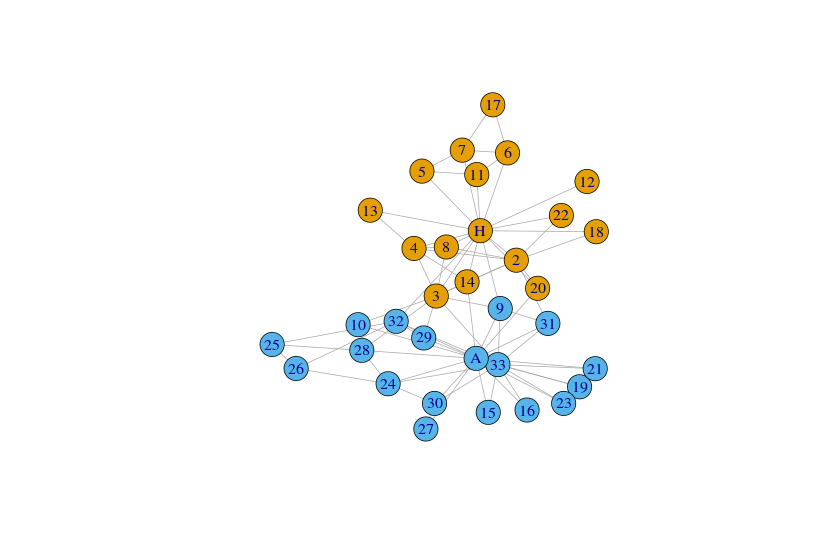
\includegraphics[width=1.20\textwidth]{ZacharysKClub.png}
\end{center}
\caption{Zachary's Karate Club}
\label{fig:zkc}
\end{figure}

To determine if the graph structure has enough information to predict the split, I used the edge betweenness algorithm as described by Girvan, Newman in their paper Community structure in social and biological networks \cite{girnewman}. In that paper they stated, that the ``betweenness of an edge as the number of shortest paths between pairs of vertices that run along it". Furthermore they state that ``edges connecting communities will have high edge betweenness" and ``by removing those edges" the communities are exposed. Now to take from Dr. Nelson's lecture \#6 ``Edge betweenness: Total amount of flow an edge carries between all pairs of nodes where a single unit of flow between two nodes divides itself evenly among all shortest paths between nodes". I believe that is straight from the Girvan Newman paper when they generalize Freeman's betweenness centrality\cite{girnewman}.
\newline

This algorithm as stated in the paper by Girvan, Newman is 
\begin{enumerate}
\item Calculate the betweenness for all edges in the network
\item Remove the edges with the highest betweenness
\item Recalculate betweenness for all edges affected by the removal
\item Repeat from step 2 until no edges remain
\end{enumerate}


In using this algorithm to find the split, I must add one caveat to step number 4, which is to stop when the number of communities desired has been reached. To know when that stopping point has been reached is easy, simply count the number of connected components in the graph. The connected components at the start of the algorithm will be one, as the original graph is one piece. When the algorithm has removed enough edges the number connected components will be increased; in short I am counting the number of connected subgraphs
 \cite{gconnect}.
\newline
I implemented this algorithm in Python using the Networkx library and can be seen in listing \ref{lst:pgn} produced the split seen in figure \ref{fig:psplit}. Please see the comments for further details. 
But stated simply the program runs as such 
\begin{enumerate}
\item Calculate the betweenness for all edges in the network
\item Get the maximum value from the dictionary gotten from edge\_betweenness\_centrality
\item Iterate through the returned dictionary and remove the edges whoes score is equal to max. This is to account for ties if any
\item Repeat until we reach the desired number of communities denoted splitTo by checking the number of connected components in the graph
\end{enumerate}

The results of my implementation can be seen in table \ref{tab:modcomp}. The actor column represents the member number from the club with actor 1 being Mr. Hi and actor 34 being John A. The following two columns show the faction and result of the split from the Zachary paper \cite{zacharykclub}. The final two columns show the faction membership as perdicted my Girvan-Newman implementation and if it matched membership correctly, hit for yes and miss for no. 

From the Zachary paper his model had a 97\% percent accuracy rating missing only 1 membership out of the 33. Whereas my model missed 4 out of the 34 resulting in a 88\% accuracy score. In comparison to the work done by Zachary I as well missed the faction that actor number 9 would go too. But it also must be noted that Girvan-Newman used the unweighted version of the Zachary graph.
\newline \newline
This model as produced by the python implementation seemed to be off, so I decided to use R to see if I did anything wrong. Why because as I went looking into graph libraries the igraph R package kept coming up so I decided to use it. 

The code used in my R implementation can be found in listing \ref{lst:rgn} and the resulting graph split in figure \ref{fig:psplit2}. Now this implementation is the most interesting. I used the igraph library and consulted the pdf reference that accompanied it on cran\cite{igraph}. In the library is this method called cluster\_edge\_betweenness which returns to us a communities object. This communities class performs the Girvan Newman algorithm for us and returns to us the edges removed, their betweenness score and much more. The comments in the code contain details on what is happening.

Since I already did the bigger analysis for my python implementation I will briefly break down the improvements. The r version correctly said the actor 9 would go to the Officers faction, actor number 14 was incorrectly placed in the Officers faction but actor 22 was correctly placed in Mr. Hi's faction. With these improvements I now miss only 2 out of the 34 resulting in a 94\% accuracy score. 
\newline
By this I can safely say that the split can be predicted with 90\% accuracy of the actual split. 


\begin{figure}
\begin{center}
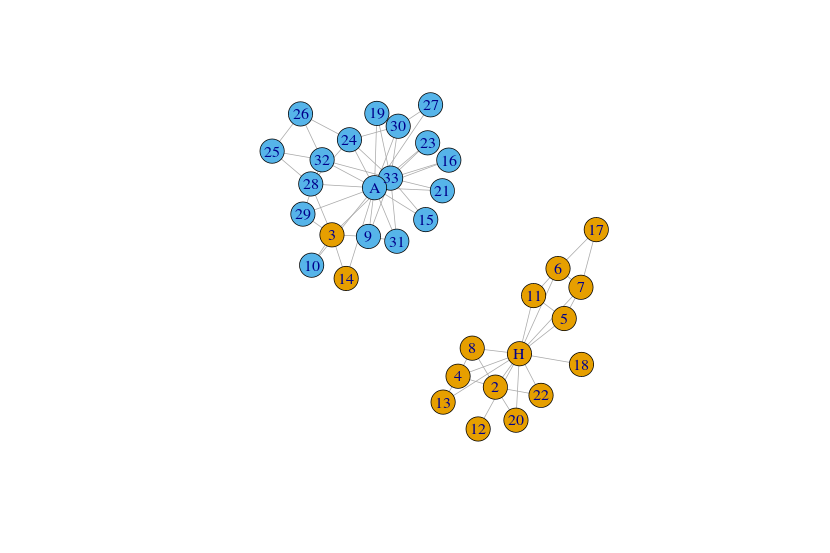
\includegraphics[scale=0.5]{RSplitClub.png}
\caption{Club split by R implementation of Girvan Newman}
\label{fig:psplit2}
\end{center}
\end{figure}

\newpage
\begin{table}
\small
\begin{tabular}{ | c | p{2cm} | p{2cm} | p{2cm} | p{2cm} | }
\hline
Actor & Faction Membership \newline From Data & Zachary\newline Membership From Split & Girvan-Newman Faction\newline Membership From Split & Hit Miss for my\newline Girvan-Newman\\
\hline
1 & Mr. Hi & Mr. Hi & Mr. Hi & Hit \\
\hline
2 & Mr. Hi & Mr. Hi & Mr. Hi & Hit \\
\hline
3 & Mr. Hi & Mr. Hi & Officer & Miss \\
\hline
4 & Mr. Hi & Mr. Hi & Mr. Hi & Hit \\
\hline
5 & Mr. Hi & Mr. Hi & Mr. Hi & Hit \\
\hline
6 & Mr. Hi & Mr. Hi & Mr. Hi & Hit \\
\hline
7 & Mr. Hi & Mr. Hi & Mr. Hi & Hit \\
\hline
8 & Mr. Hi & Mr. Hi & Mr. Hi & Hit \\
\hline
9 & Mr. Hi & Officers & Officers & Miss \\
\hline
10 & Officers & Officers & Mr. Hi & Miss \\
\hline
11 & Mr. Hi & Mr. Hi & Mr. Hi & Hit \\
\hline
12 & Mr. Hi & Mr. Hi & Mr. Hi & Hit \\
\hline
13 & Mr. Hi & Mr. Hi & Mr. Hi & Hit \\
\hline
14 & Mr. Hi & Mr. Hi & Mr. Hi & Hit \\
\hline
15 & Officers & Officers & Officers & Hit \\
\hline
16 & Officers & Officers & Officers & Hit \\
\hline
17 & Mr. Hi & Mr. Hi & Mr. Hi & Hit \\
\hline
18 & Mr. Hi & Mr. Hi & Mr. Hi & Hit \\
\hline
19 & Officers & Officers & Officers & Hit \\
\hline
20 & Mr. Hi & Mr. Hi & Mr. Hi & Hit \\
\hline
21 & Officers & Officers & Officers & Hit \\
\hline
22 & Mr. Hi & Mr. Hi &  Officers & Miss \\
\hline
23 & Officers & Officers & Officers & Hit \\
\hline
24 & Officers & Officers & Officers & Hit \\
\hline
25 & Officers & Officers & Officers & Hit \\
\hline
26 & Officers & Officers & Officers & Hit \\
\hline
27 & Officers & Officers & Officers & Hit \\
\hline
28 & Officers & Officers & Officers & Hit \\
\hline
29 & Officers & Officers & Officers & Hit \\
\hline
30 & Officers & Officers & Officers & Hit \\
\hline
31 & Officers & Officers & Officers & Hit \\
\hline
32 & Officers & Officers & Officers & Hit \\
\hline
33 & Officers & Officers & Officers & Hit \\
\hline
34 & Officers & Officers & Officers & Hit \\
\hline
\end{tabular}
\caption{Comparisons of the results of split as generated by my Girvan Newman implementation to Zachary's predictions and the actual data as was done in the original paper}
\label{tab:modcomp}
\end{table}



\begin{figure}
\begin{center}
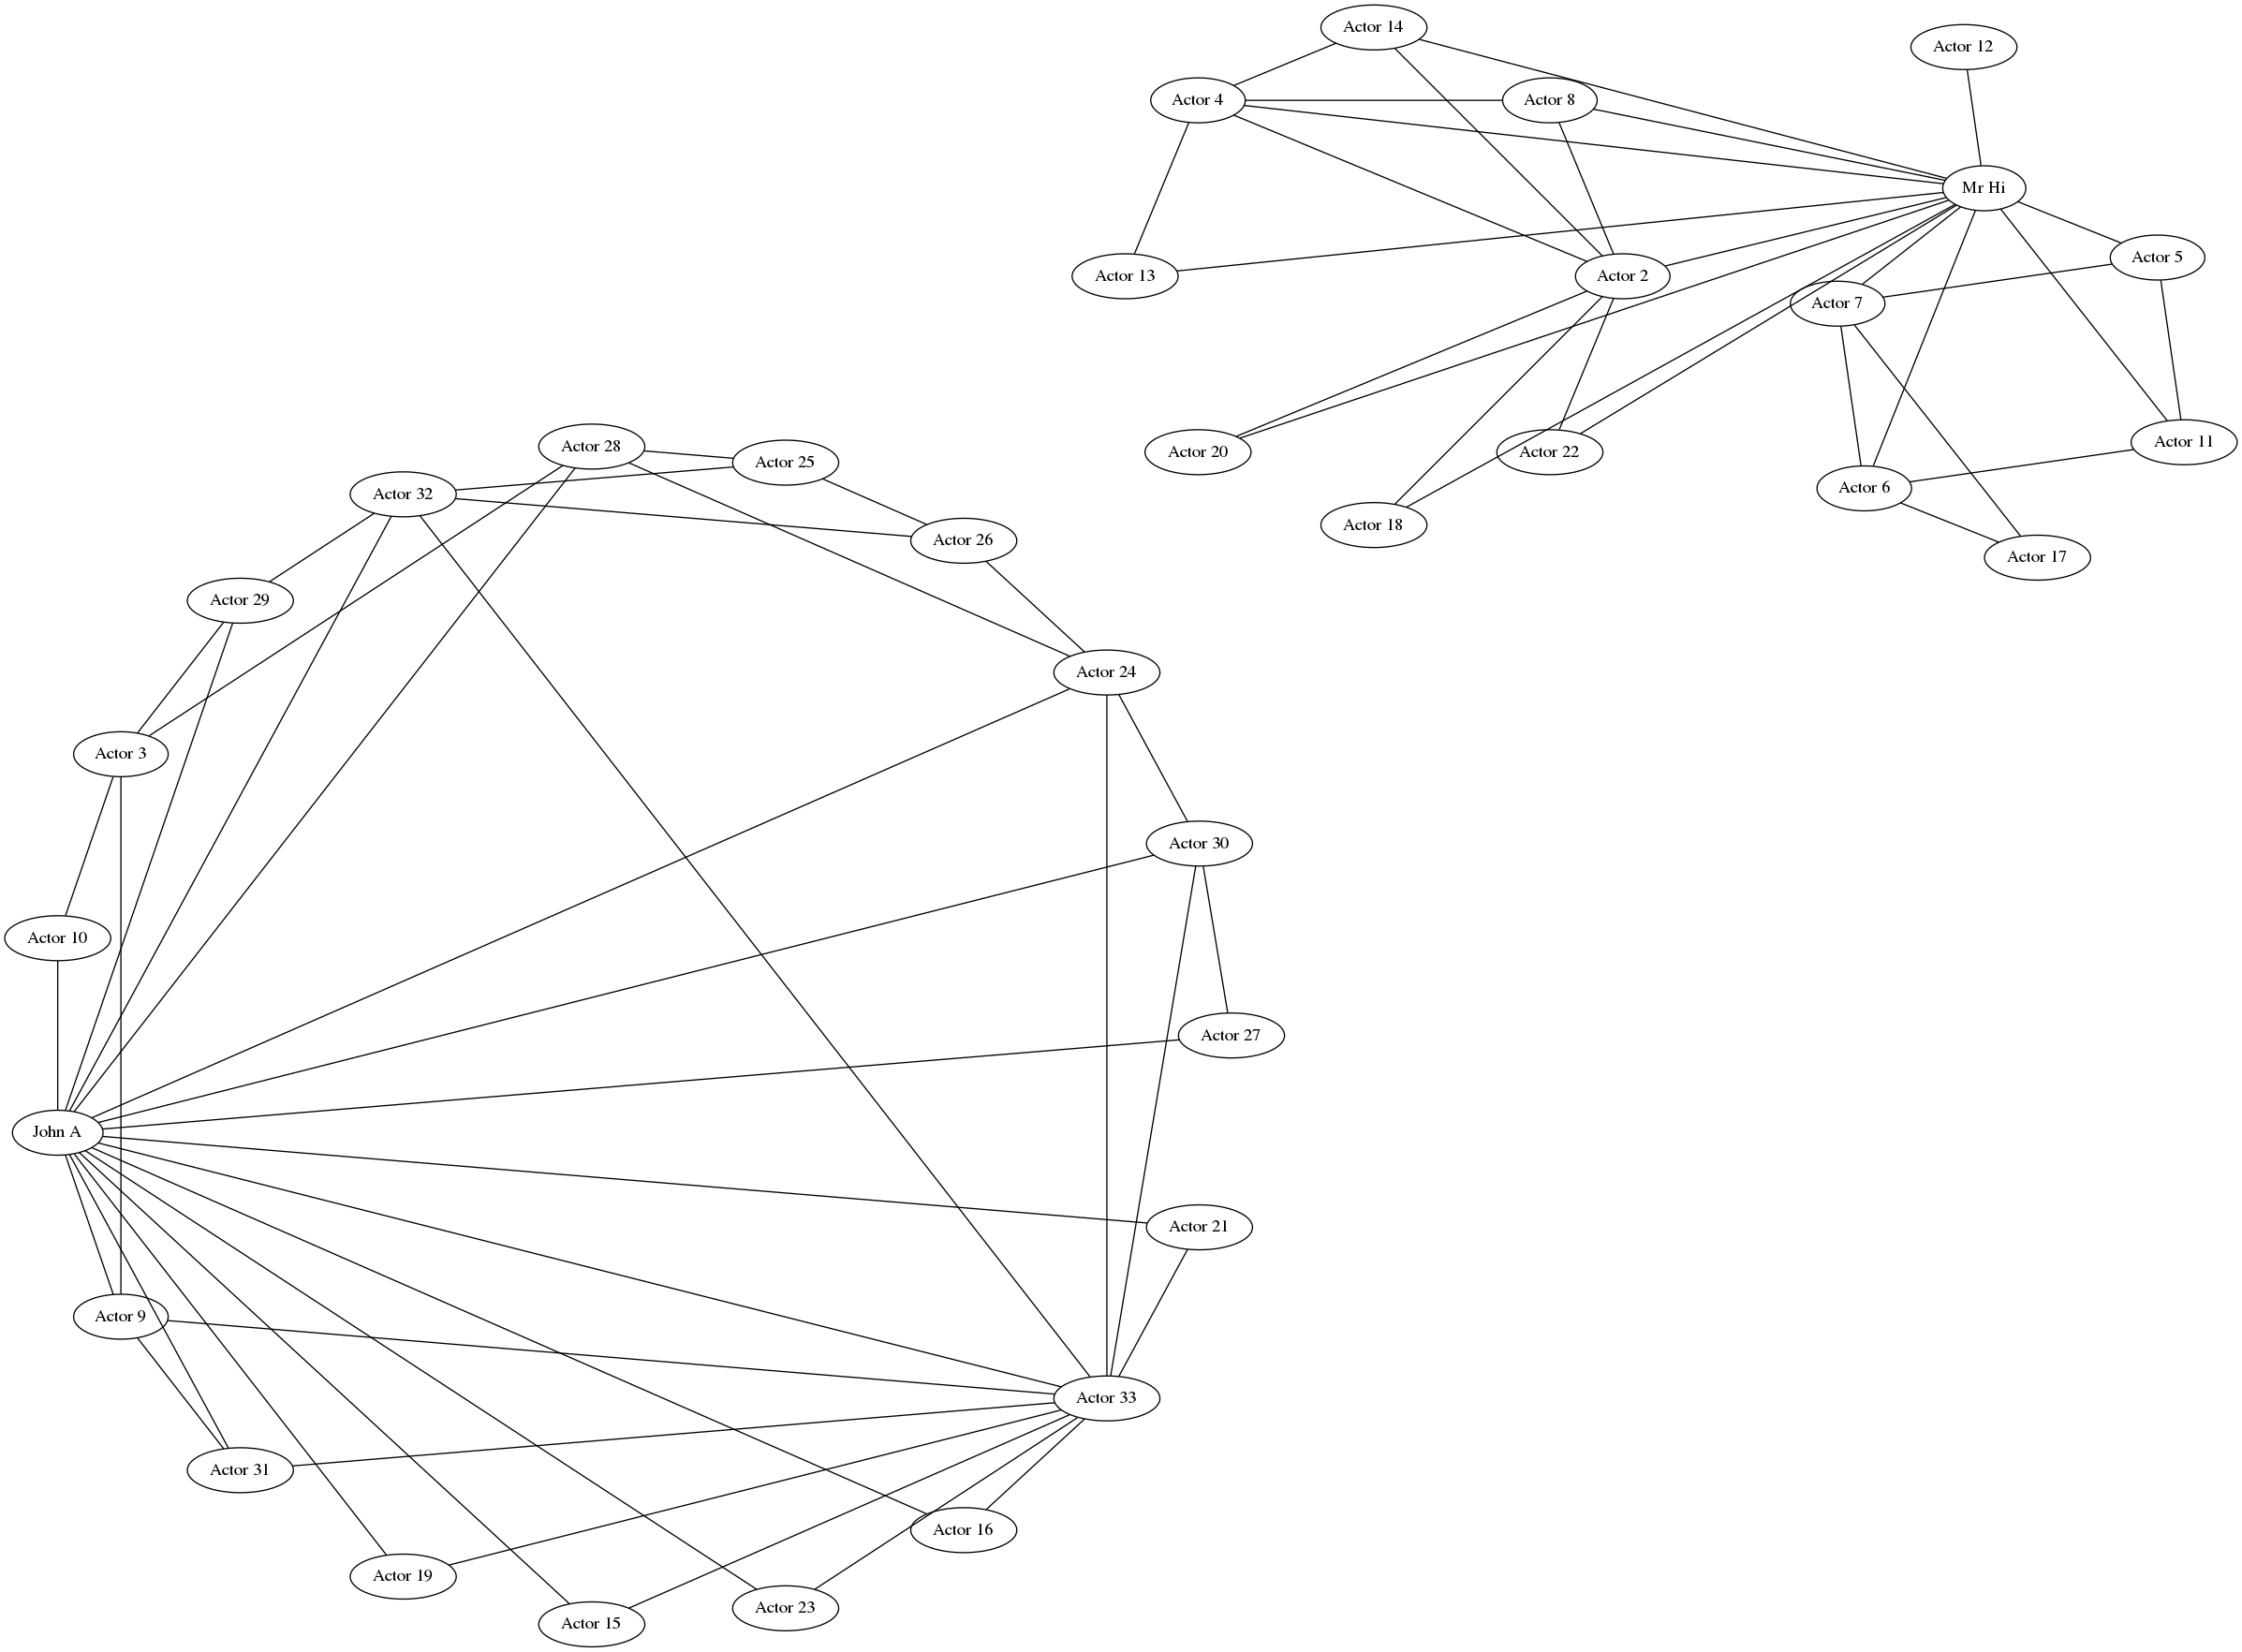
\includegraphics[scale=0.2]{supportingMaterials/weightedkclub/kc.png}
\caption{Club split by my implementation of Girvan Newman}
\label{fig:psplit}
\end{center}
\end{figure}

\newpage
\lstinputlisting[language=Python,frame=single,
caption={Girvan Newman edge betweenness centrality},label=lst:pgn,captionpos=b]{kclub.py}
\newpage
\begin{lstlisting}[frame=single,caption={Convert dot files to png}]
$ circo -Tpng -o kc.png kc2.dot
$ circo -Tpng -o kc3.png  kc3.dot
$ circo -Tpng -o kc4.png  kc4.dot
$ circo -Tpng -o kc5.png  kc5.dot
\end{lstlisting}
\newpage
\lstinputlisting[language=R,frame=single,
caption={Girvan Newman edge betweenness centrality in R},label=lst:rgn,captionpos=b]{karateClub.R}
\newpage

\section*{2}
\subsection*{Question}

\begin{verbatim}
2.  We know the group split in two different groups.  Suppose the
disagreements in the group were more nuanced -- what would the clubs
look like if they split into groups of 3, 4, and 5?

\end{verbatim}

\subsection*{Answer}
Using the same R code as in the second implementation I changed the splitTo value to 3 communities figure \ref{fig:3way},4 communities figure\ref{fig:4way}, and 5 communities figure\ref{fig:5way}. Those figures are seen below.

\begin{figure}[h]
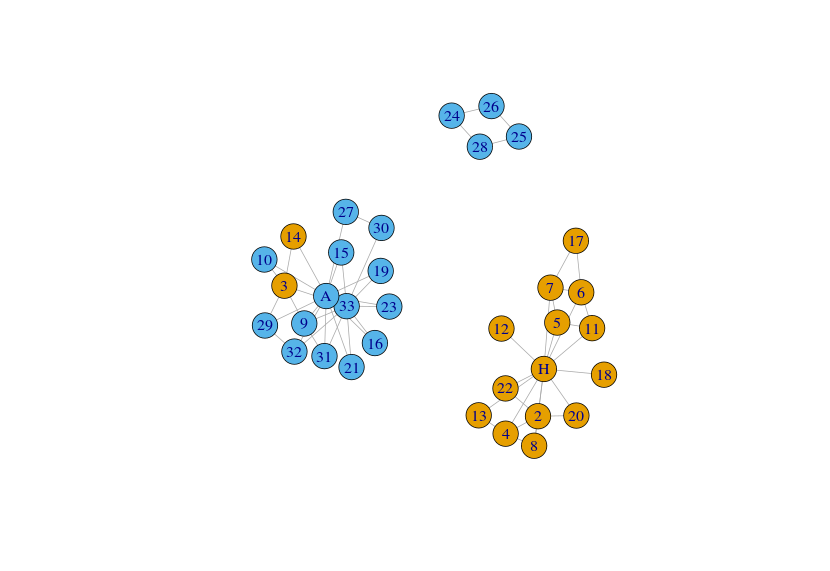
\includegraphics[scale=0.5]{clubSplit3.png}
\caption{Karate Club Graph Split Into 3 Communities}
\label{fig:3way}
\end{figure}

\begin{figure}
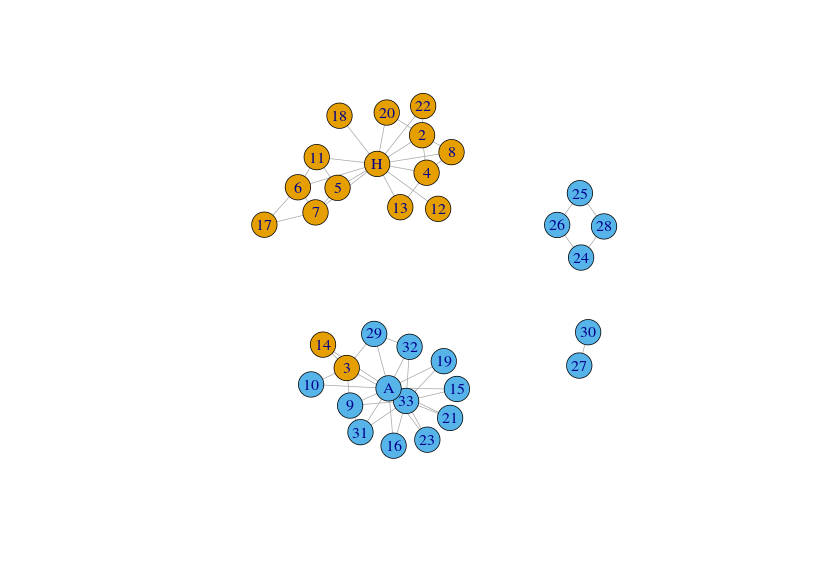
\includegraphics[scale=0.5]{clubSplit4.png}
\caption{Karate Club Graph Split Into 4 Communities}
\label{fig:4way}
\end{figure}

\begin{figure}
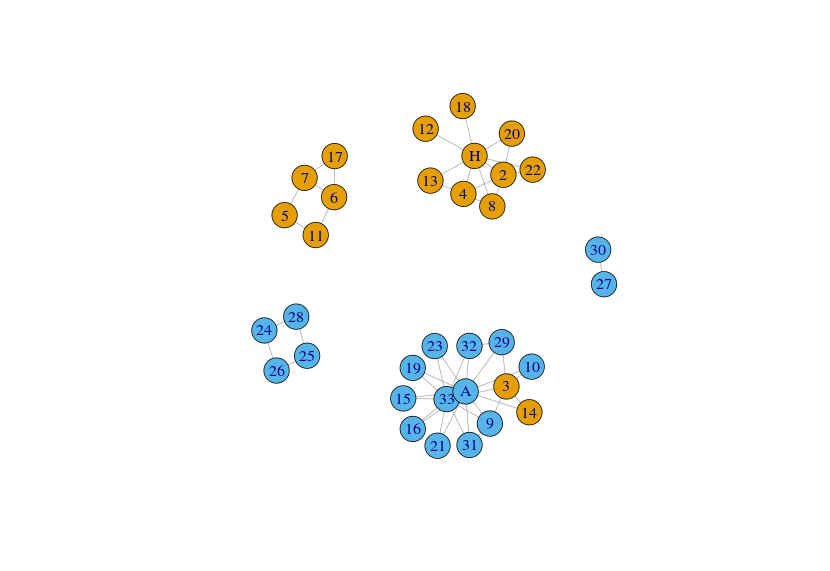
\includegraphics[scale=0.5]{clubSplit5.png}
\caption{Karate Club Graph Split Into 5 Communities}
\label{fig:5way}
\end{figure}
\newpage
\bibliographystyle{acm}
\bibliography{references}        
\end{document}
